\documentclass{beamer}
\usepackage{beamerthemeshadow}
\usepackage{color}
\usepackage[all]{xy}


%%%% choose your presentation style:
\mode<presentation>
{
  \usetheme{Copenhagen} %%%
 \usecolortheme{beaver}

%%% set style for ovelays: lists (and other text) appearing one item at a time
%%% This will create a dimmed preview of next item:
\setbeamercovered{transparent}
%%% This will hide it entirely:
%\setbeamercovered{invisible}
}
%% if you don't want page numbers to show: 
\setbeamertemplate{footline}[page number]{}


\begin{document}
\title{Sample Beamer presentation}
\author{Elena Machkasova}
\institute[UMM] % (optional, but mostly needed)
{
 % \inst{1}%
  University of Minnesota, Morris
}
\date[]  
{HHMI lunch meeting, June 10 2015}

\begin{frame}
  \titlepage
\end{frame}

\begin{frame}

  \frametitle{Outline}
\tableofcontents
\end{frame}

\section{Main elements of Beamer slides}

\subsection{Math formulas}

\begin{frame}
  \frametitle{Text, fonts, and formulas}
Here is some text on my slide. 

If I want, I can set up some formulas:
$$
E = mc^2.
$$

This is \alert{important}:
\[
e = \lim_{n \to \infty} {\left( 1 + \frac{1}{n} \right)}^n
\]

You can also use \textbf{boldface} and \textit{italics}. 
\end{frame}

\subsection{Simple lists}

\begin{frame}
  \frametitle{How to set up lists}
Unordered lists:
\begin{itemize}
\item First item 
\item Second item
\item Third item
\end{itemize}
\end{frame}

\begin{frame}
  \frametitle{How to set up lists}
Ordered lists:
\begin{enumerate}
\item First item 
\item Second item
\item Third item
\end{enumerate}
\end{frame}

\begin{frame}
  \frametitle{How to add pictures}
\begin{figure}
%%% note: the file is in the same folder as your .tex file
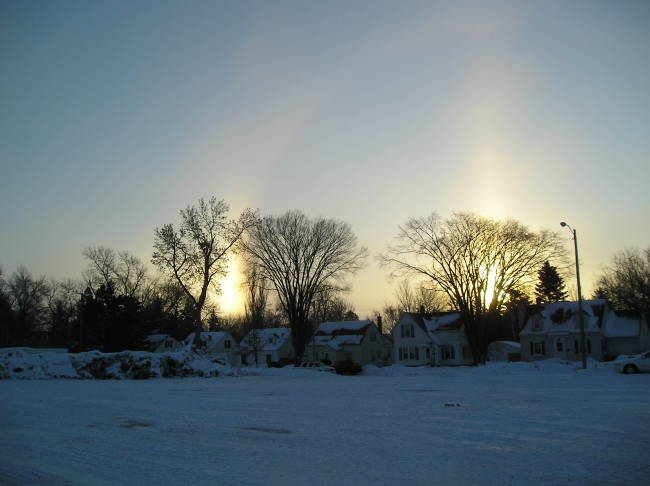
\includegraphics[height=45mm]{halo.jpg}
\end{figure}

Here we can see halo. 
\end{frame}

\section{Making items appear one by one}

\begin{frame}
  \frametitle{Simple overlays}
\begin{itemize}
\item First item 
\pause
\item Second item
\pause
\item Third item
\end{itemize}
\end{frame}

\begin{frame}
\frametitle{More control over when items appear}
\begin{itemize}
\item <1-> First slide
\item <3> Third slide
\item <2>Second slide only
\item <1->Also first slide
\end{itemize}
\end{frame}

\section{showing program code}

%%% If you are including verbatim text, make the frame fragile
\begin{frame}[fragile]
\frametitle{Including text verbatim}
Typically you include porgram code verbatim:
\begin{verbatim}
(defn get-match-name [fname]
  "extract a function name from a qualified name"
  (let [m (nth (re-matches #"(.*)\$(.*)" fname) 2)
        matched (if m m (nth (re-matches #"(.*)/(.*)" 
            fname) 2))]
    (if matched
      (check-if-anonymous-function 
           (lookup-funct-name matched))
      fname)))
\end{verbatim}
\end{frame}

\begin{frame}
  \frametitle{Discussion}
Questions?
\end{frame}

\end{document}
